 \documentclass[tikz,border=2mm]{standalone}
\begin{document}
	\tikzset{>=latex}
	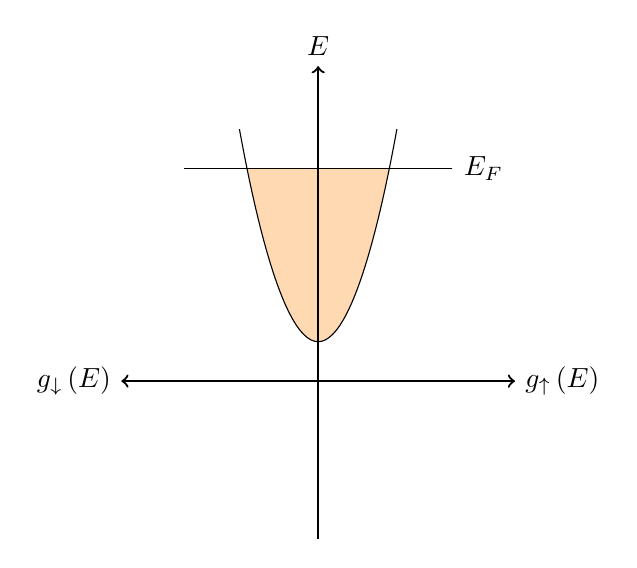
\begin{tikzpicture}
		\shade[top color=orange!30!white,bottom color=orange!30!white] 
		(0,0.5) parabola (0.9,2.7) |- (0,2.7);
		\shade[top color=orange!30!white,bottom color=orange!30!white] 
		(0,0.5) parabola (-0.9,2.7) |- (0,2.7);
		
		\draw[->=stealth, thick] (0,0)--(2.5,0) node[right]            {$g_\uparrow\left(E\right)$};
		\draw[->=stealth, thick] (0,0)--(-2.5,0) node[left]            {$g_\downarrow\left(E\right)$};
		\draw[->=stealth, thick] (0,-2)--(0,4) node[above]{$E$};
		
		\draw (0,0.5) parabola (1,3.2);
		\draw (1.7,2.7) -- (0,2.7);   
		\draw (0,0.5) parabola (-1,3.2);
		\draw (-1.7,2.7) -- (0,2.7);
		\node[] at (2.1,2.7) {$E_F$};
	\end{tikzpicture}
\end{document}

% See - https://www.latex4technics.com/?note=ohq